\documentclass{if-beamer}
\begin{document}
	
	\title[Campus Formoso do Araguaia]{Configuração de Redes e Servidores}
	\subtitle{Aula 2 }
	\author{Gilmar Gomes do Nascimento}
	\institute[IFTO]{
		Instituto Federal do Tocantins\\
		Campus Formoso do Araguaia
	}
	\date{\today}
	\logo{
		
\includegraphics[scale=0.0085]{logo.jpg}
	}
	\subject{Servers} % metadata
	
	\graphicspath{{figuras/}}
	%---------------------------------------------------------------------------------
	
	\begin{frame}
		\titlepage
	\end{frame}
	
	% ============================================================
% SERVIDORES (SISTEMAS OPERACIONAIS)
% ============================================================

\begin{frame}{Servidores (Sistemas Operacionais)}
\begin{figure}
		
\includegraphics[scale=0.89]{server-os-comparison}
	\end{figure}
\end{frame}

\begin{frame}
	\begin{block}{Principais sistemas operacionais para servidores}
		\begin{itemize}
			\item \textbf{Microsoft Windows Server} – Ecossistema empresarial e integração com Active Directory
			\item \textbf{macOS Server} – Descontinuado, mas ainda utilizado em ambientes legados
			\item \textbf{Linux Server} – Ampla variedade de distribuições (comunitárias e empresariais)
			\item \textbf{FreeBSD} –  Performance e Estabilidade
			\item \textbf{OpenBSD} -- A Segurança em Primeiro Lugar
		\end{itemize}
	\end{block}
	
\end{frame}

% ============================================================
% WINDOWS SERVER
% ============================================================

\begin{frame}[allowframebreaks]{Windows Server}
	\begin{block}{O que é o Windows Server?}
		O Windows Server é a plataforma de servidor empresarial da Microsoft que permite
		que as organizações executem e protejam aplicativos, serviços e cargas de trabalho
		em ambientes locais, híbridos e de nuvem.
	\end{block}
	
	\framebreak
	
	\begin{block}{Características principais}
		Windows Server fornece a base para a computação segura, escalonável e de alto 
		desempenho que cresce com sua organização. Baseado em décadas de inovação do Windows, ele serve como backbone para milhões de organizações em todo o mundo, alimentando tudo, desde servidores de arquivos e aplicativos Web até cargas de trabalho corporativas complexas e soluções orientadas por IA. \\
	\end{block}
\framebreak	
	\begin{block}{Diferenciais do Windows Server}
		\begin{itemize}
			\item \textbf{Ambientes mistos}: gerenciamento unificado de cargas de trabalho do Windows, Linux e contêiner.
			\item \textbf{Integração empresarial}: integração perfeita com o SQL Server, o System Center, o Exchange, o SharePoint, o Project e a infraestrutura existente do Windows.
		\end{itemize}
		\end{block}
\framebreak
\begin{block}{Diferenciais do Windows Server}
\begin{itemize}
			\item \textbf{Suporte comercial}: suporte de nível empresarial com uma comunidade de tecnologia ativa.
			\item \textbf{Cenários de conformidade}: recursos internos para setores regulamentados (saúde, finanças, governo).
			\item \textbf{Licenciamento flexível}: escolha entre licenciamento pago conforme o uso, perpétuo ou baseado em assinatura.
		\end{itemize}
	\end{block}
	
	\framebreak
	
	\begin{figure}
		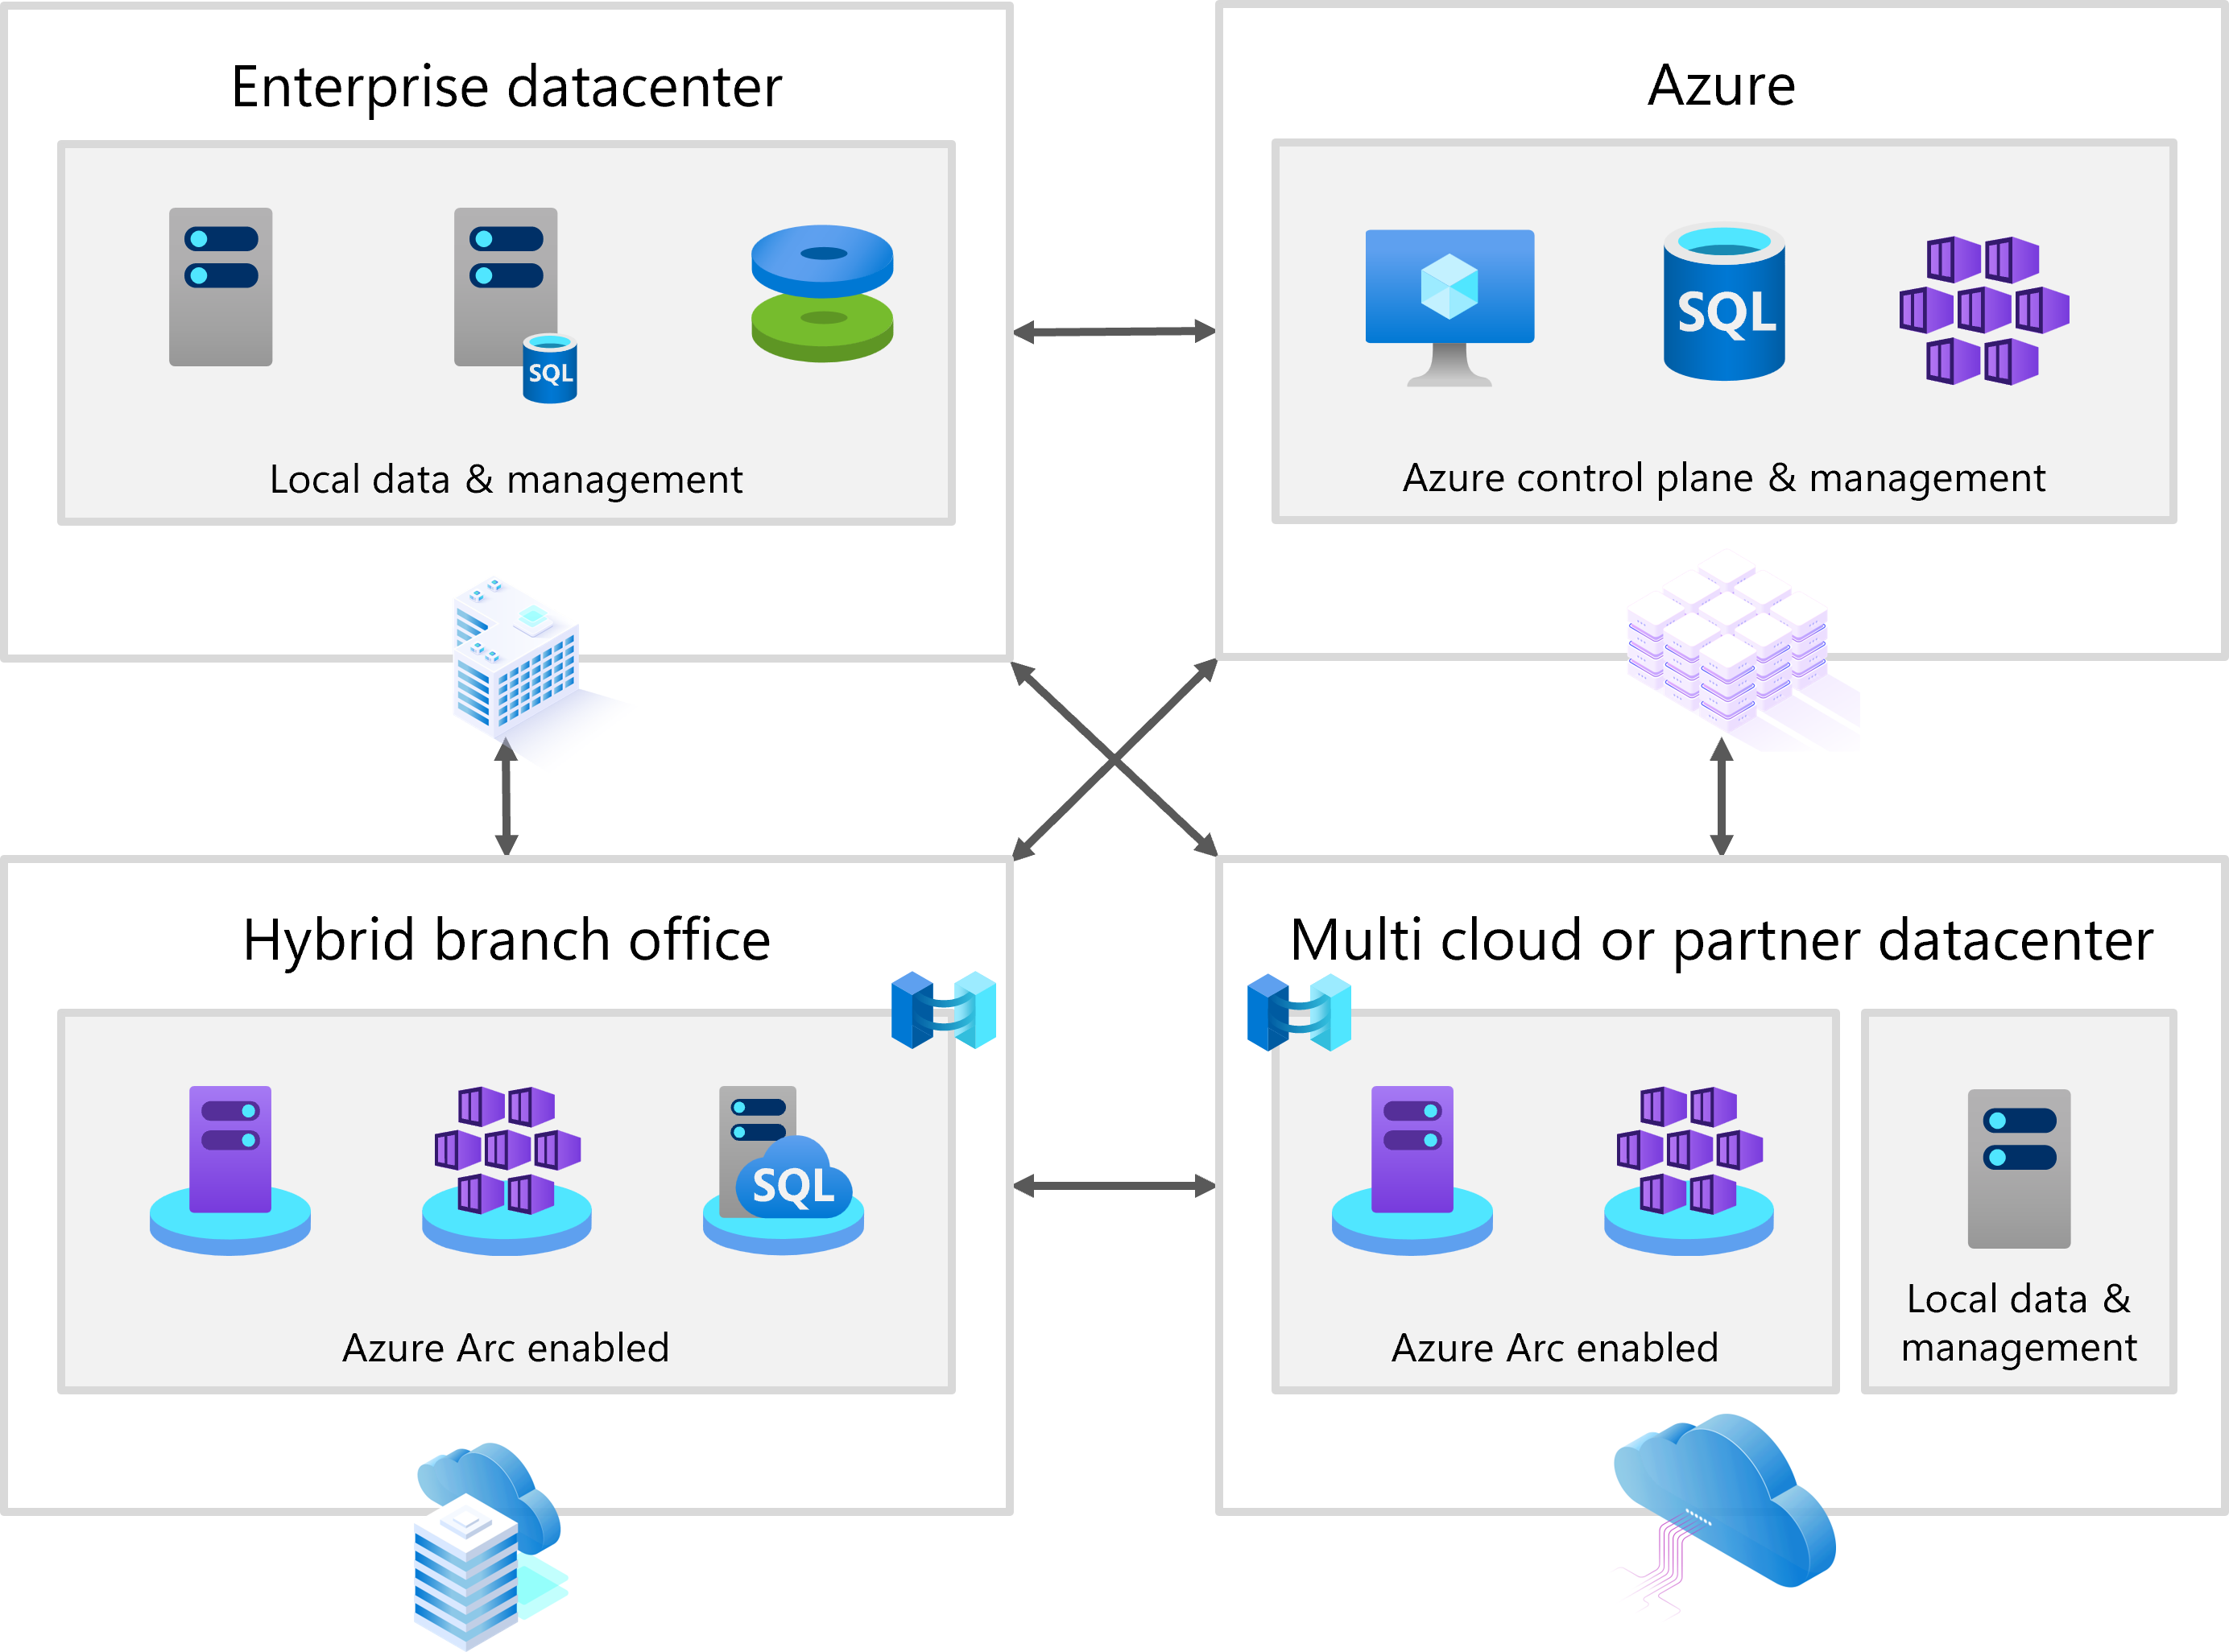
\includegraphics[scale=0.35]{ms-windows-servers}
	\end{figure}
	
	\framebreak
	
	\begin{figure}
		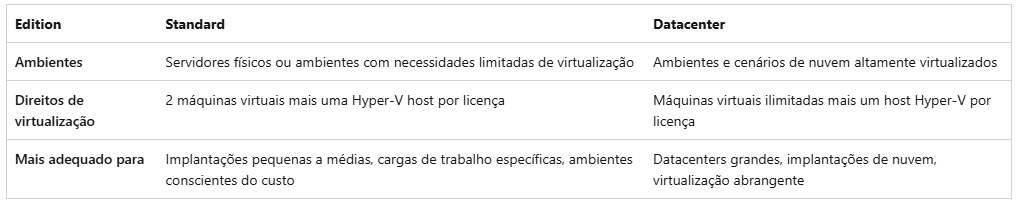
\includegraphics[scale=0.5]{windows-server-edition}
	\end{figure}
\end{frame}

% ============================================================
% MACOS SERVER
% ============================================================

\begin{frame}[allowframebreaks]{MacOS Server}
	\begin{block}{O que foi o macOS Server?}
		O macOS Server era uma plataforma de servidor da Apple, projetada para integrar-se perfeitamente ao ecossistema Apple. Era utilizado principalmente para gerenciamento de dispositivos (MDM), servidores de arquivos, e serviços de rede em ambientes corporativos com predominância de Macs.
	\end{block}
	
	\framebreak
	
	\begin{block}{Descontinuação}
		Desde 21 de abril de 2022, a Apple descontinuou o macOS Server. Clientes atuais do macOS Server ainda podem baixar e usar o app com o macOS Monterey.
		
		\vspace{0.3cm}
		A partir de 29 de outubro de 2024, o Profile Manager não poderá mais criar ou renovar certificados de notificação \textit{push} para gerenciamento de dispositivos. No entanto, certificados existentes continuarão funcionando.
	\end{block}
	
	\framebreak
	
	\begin{block}{Alternativas ao macOS Server}
		Para organizações que dependiam do macOS Server, as principais alternativas incluem:
		\begin{itemize}
			\item \textbf{Jamf Pro} – Solução líder em gerenciamento de dispositivos Apple
			\item \textbf{Mosyle} – MDM focado em educação e empresas
			\item \textbf{Kandji} – MDM moderno para Apple no ambiente corporativo
			\item \textbf{Microsoft Intune} – Gerenciamento unificado para múltiplos sistemas
		\end{itemize}
	\end{block}
\end{frame}

% ============================================================
% LINUX SERVERS
% ============================================================

\begin{frame}[allowframebreaks]{Linux Servers}
	\begin{block}{O que é um servidor Linux?}
		O Linux é um sistema operacional de código aberto amplamente utilizado em servidores devido à sua estabilidade, segurança, flexibilidade e baixo custo. Existem centenas de distribuições, divididas principalmente entre \textbf{empresariais} e \textbf{comunitárias}.
	\end{block}
	\begin{figure}
		
\includegraphics[scale=0.4]{linux-para-servidores}
	\end{figure}
	\framebreak
	\begin{block}{Principais distribuições}
		\begin{itemize}
			\item \textbf{Debian} – Estável, comunitária, base para o Ubuntu
			\item \textbf{Ubuntu Server} – Ampla documentação, fácil de usar
			\item \textbf{Red Hat Enterprise Linux (RHEL)} – Empresarial, suporte pago
			\item \textbf{SUSE Linux Enterprise} – Empresarial, forte na Europa
			\item \textbf{Fedora Server} – Inovadora, ciclo curto de atualizações
			\item \textbf{Rocky Linux} / \textbf{AlmaLinux} – Sucessores do CentOS (estáveis e gratuitos)
		\end{itemize}
	\end{block}
\end{frame}

% ============================================================
% DIFERENÇA ENTRE DISTRIBUIÇÕES LINUX
% ============================================================

\begin{frame}[allowframebreaks]{Diferença entre distribuições Linux}
	\begin{block}{Distribuições empresariais}
		\begin{itemize}
			\item Oferecem \textbf{suporte técnico pago} (com contratos de nível de serviço)
			\item Acesso a \textbf{ferramentas de gerenciamento} proprietárias
			\item Certificação para \textbf{hardware específico}
			\item Exemplos: Red Hat Enterprise Linux, SUSE Linux Enterprise, Ubuntu Pro
		\end{itemize}
	\end{block}
	
	\framebreak
	
	\begin{block}{Distribuições comunitárias}
		\begin{itemize}
			\item Suporte baseado em \textbf{comunidade, fóruns e documentação}
			\item Código aberto e gratuito
			\item Atualizações frequentes e rápida inovação
			\item Exemplos: Debian, Fedora, Arch Linux, Rocky Linux
		\end{itemize}
	\end{block}
\end{frame}

% ============================================================
% COMPARAÇÃO ENTRE SOs PARA SERVIDORES
% ============================================================

%\begin{frame}{Comparação entre SOs para servidores}
%	\begin{table}
%		\centering
%		\small
%		\begin{tabular}{|p{2.5cm}|p{2.5cm}|p{2.5cm}|p{2.5cm}|}
%			\hline
%			\textbf{Característica} & \textbf{Windows Server} & \textbf{macOS Server} & \textbf{Linux Server} \\
%			\hline
%			Custo & Pago (licenciamento) & Descontinuado (gratuito até 2022) & Gratuito (maioria) \\
%			\hline
%			Suporte & Microsoft (pago) & Descontinuado & Comunidade ou pago (RHEL, SUSE) \\
%			\hline
%			Facilidade de uso & Interface gráfica robusta & Integração Apple & Linha de comando (maioria) \\
%			\hline
%			Segurança & Bom, com atualizações regulares & Bom, com foco em privacidade & Excelente, com auditoria aberta \\
%			\hline
%			Casos de uso & AD, Exchange, SQL Server, IIS & Gerenciamento Apple, servidores de rede & Web, banco de dados, contêineres, DevOps \\
%			\hline
%		\end{tabular}
%	\end{table}
%\end{frame}

% ============================================================
% REFERÊNCIAS
% ============================================================

\begin{frame}[allowframebreaks]{Referências}
	\begin{thebibliography}{9}
		\bibitem{microsoft-windows-server}
		MICROSOFT. \textit{Windows Server Documentation}. Disponível em: \url{https://learn.microsoft.com/en-us/windows-server/}. Acesso em: 26 de agosto de 2026.
		
		\bibitem{apple-macos-server}
		APPLE. \textit{macOS Server - About the discontinuation}. Disponível em: \url{https://support.apple.com/macos-server}. Acesso em: 26 de agosto de 2026.
		
		\bibitem{red-hat}
		RED HAT. \textit{Red Hat Enterprise Linux Documentation}. Disponível em: \url{https://access.redhat.com/documentation/en-us/red_hat_enterprise_linux/}. Acesso em: 26 de agosto de 2026.
		
		\bibitem{ubuntu-server}
		CANONICAL. \textit{Ubuntu Server Documentation}. Disponível em: \url{https://ubuntu.com/server/docs}. Acesso em: 26 de agosto de 2026.
		
		\bibitem{rocky-linux}
		ROCKY LINUX. \textit{Rocky Linux Documentation}. Disponível em: \url{https://docs.rockylinux.org/}. Acesso em: 26 de agosto de 2026.
		\bibitem{freebsd}
		FREEBSD. \textit{FreeBSD Documentation}. Disponível em: \url{https://www.freebsd.org/doc/}. Acesso em: 26 de agosto de 2026.
		
		\bibitem{openbsd}
		OPENBSD. \textit{OpenBSD Documentation}. Disponível em: \url{https://www.openbsd.org/}. Acesso em: 26 de agosto de 2026.
		
		\bibitem{bsd-vs-linux}
		BSD VS LINUX. \textit{Differences between BSD and Linux}. Disponível em: \url{https://www.over-yonder.net/~fullermd/rants/bsd4linux/}. Acesso em: 26 de agosto de 2026.
		
		\bibitem{netflix-freebsd}
		NETFLIX. \textit{Netflix and FreeBSD}. Disponível em: \url{https://netflixtechblog.com/freebsd-at-netflix}. Acesso em: 26 de agosto de 2026.
	\end{thebibliography}
\end{frame}

\begin{frame}{Configuração de redes e servidores}
\begin{figure}
	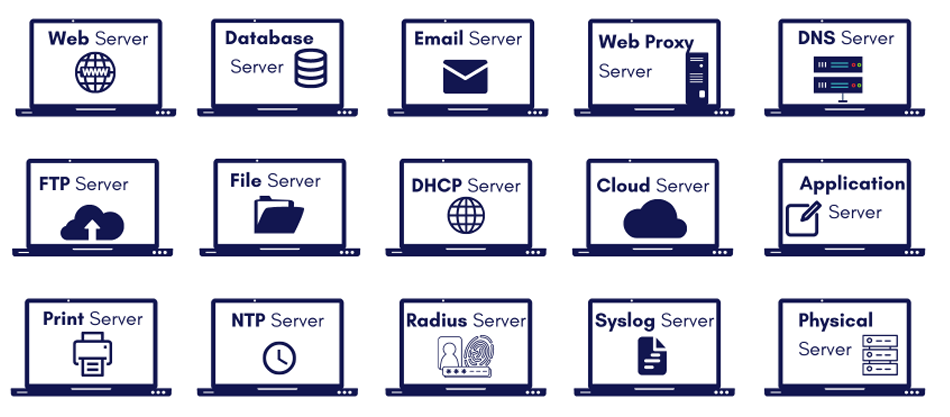
\includegraphics[scale=0.57]{servers}
\end{figure}
\end{frame}


	\begin{frame}{Logs}
\begin{quote}
Em computação, log de dados é uma expressão utilizada para descrever o processo de registro de eventos relevantes num sistema computacional. Esse registro pode ser utilizado para restabelecer o estado original de um sistema ou para que um administrador conheça o seu comportamento no passado.
\end{quote}
\end{frame}

\begin{frame}[allowframebreaks]{Taxonomia de Logs (Gu et al., 2022)}
    \begin{block}{Uma visão estruturada sobre logging}
        Segundo a taxonomia proposta por Gu et al. (2022), o ecossistema de logs pode ser compreendido por meio de oito conceitos inter-relacionados, que vão desde a prática de registro até os artefatos gerados.
    \end{block}
\framebreak    
    \begin{table}
        \centering
        \small
        \begin{tabular}{|p{2.8cm}|p{8.5cm}|}
            \hline
            \textbf{Conceito} & \textbf{Descrição Geral} \\
            \hline
            \texttt{Logging Practice} & A abordagem geral e as estratégias adotadas pela equipe para implementar logs no sistema [citation:2]. \\
            \hline
            \texttt{Logging} & O ato de registrar informações durante a execução de um software [citation:2]. \\
            \hline
            \texttt{Log Statement} & A instrução no código-fonte que gera um log (ex: `logger.info("Mensagem")`). \\
            \hline
            \texttt{Log Message} & A mensagem gerada por um \texttt{Log Statement} em tempo de execução. \\
            \hline
        \end{tabular}
    \end{table}
    \framebreak
            \begin{table}
        \centering
        \small
        \begin{tabular}{|p{2.8cm}|p{8.5cm}|}            
            \hline
            \texttt{Log} & O registro individual, contendo uma \texttt{Log Message}, data/hora e nível de severidade. \\
            \hline
            \texttt{Log Content} & Os dados específicos incluídos em uma \texttt{Log Message} (ex: ID do usuário, resultado de uma operação). \\
            \hline
            \texttt{Log Level} & A severidade do evento (ex: INFO, WARN, ERROR), que orienta a relevância do log [citation:2]. \\
            \hline
            \texttt{Log Placement} & A localização no código onde um \texttt{Log Statement} é inserido (a decisão de "onde logar") [citation:2]. \\
            \hline
            \texttt{Log Location} & O destino onde os logs são armazenados (ex: arquivo, servidor central, banco de dados). \\
            \hline
        \end{tabular}
    \end{table}
\end{frame}


\begin{frame}
\begin{block}{Registro automático}
Um log é um registro automático e cronológico de eventos gerados por um sistema, software ou rede.

\end{block}
\end{frame}


\begin{frame}{O que é um log?}
\begin{itemize}
\item \textbf{Registro de eventos:} Documenta o que aconteceu, quem fez e quando ocorreu
\item \textbf{Estrutura básica:} Contém data/hora, nível de severidade e uma descrição do fato
\item \textbf{Imutabilidade:} Salva o histórico exato para auditoria e segurança
\end{itemize}

\end{frame}	

\begin{frame}{Para quem servem?}
\begin{itemize}
\item \textbf{Depuração(Debugging):} Ajudam a achar a origem dos erros e falhas rapidamente
\item \textbf{Monitoramento:} Permitem observar a saúde da aplicação em tempo real
\item \textbf{Auditoria e Segurança:} Rastreiam ações de usuários e acessos indevidos
\end{itemize}

\end{frame}

\begin{frame}[allowframebreaks]{Logs no Windows}
	\begin{block}{Visualizador de eventos}
		Pressione \texttt{Win + R}, digite \texttt{eventvwr.msc} e pressione Enter para abrir o Visualizador de Eventos.
	\end{block}
	
	\framebreak
	
		\begin{figure}
			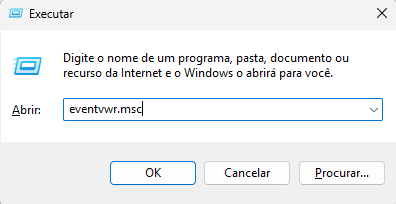
\includegraphics[scale=1]{eventvwr}
		\end{figure}		

	\framebreak
	
		\begin{figure}
			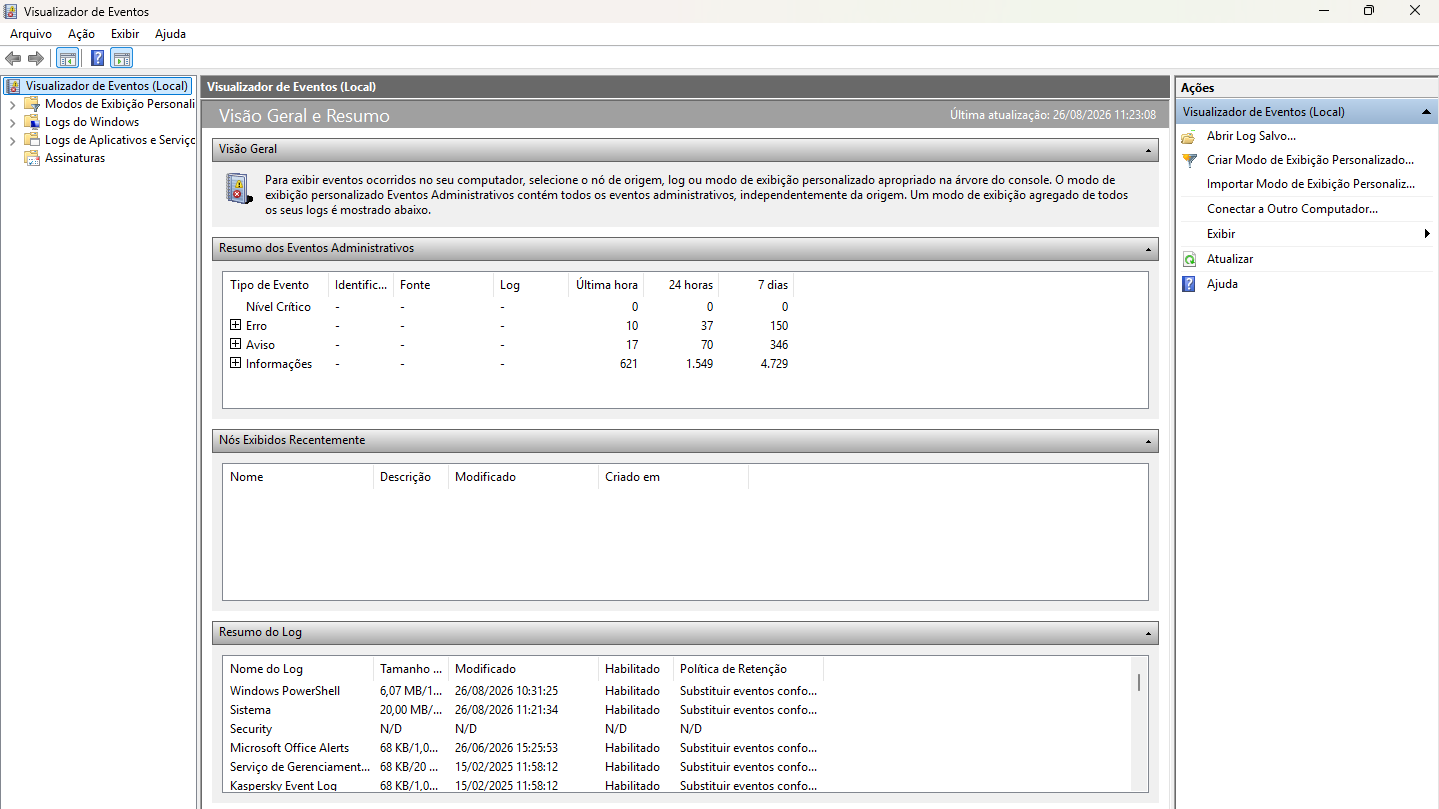
\includegraphics[scale=0.3]{viewer-events}
		\end{figure}
\newpage
	\framebreak

	No painel esquerdo, navegue até Logs de Aplicações e Serviços $\rightarrow$ Microsoft $\rightarrow$ Windows $\rightarrow$ DriverFrameworks-UserMode $\rightarrow$ Operacional.
	
	Se este log estiver desativado, clique com o botão direito sobre ele e selecione Habilitar Log.
	
	Para filtrar apenas os eventos de conexão do pen drive, procure por eventos com os IDs 2003 ou 2100. O evento 2003 é um dos mais comuns para identificar a conexão de um dispositivo de armazenamento USB.
	
	\framebreak
	
	\begin{block}{Analisando o Registro do Windows (Histórico Completo)}
		O sistema guarda um registro persistente de todos os dispositivos USB que já foram conectados, como uma ``assinatura'' de cada um. As principais chaves do Registro para isso são:
	\end{block}
	
	\framebreak
		\texttt{HKLM\textbackslash SYSTEM\textbackslash CurrentControlSet\textbackslash Enum\textbackslash USBSTOR}: Armazena informações detalhadas sobre dispositivos de armazenamento USB que já foram conectados. Dentro dela, você encontra subchaves com o ID do Dispositivo (que revela o fabricante e o produto) e o Número de Série do pen drive.
	
	\framebreak
	
	Dentro da chave do dispositivo, subchaves com os nomes 0064, 0066 e 0067 podem conter timestamps da primeira conexão (0064), da última conexão (0066) e da última remoção (0067).
	\framebreak
	\texttt{HKLM\textbackslash SYSTEM\textbackslash MountedDevices}: Esta chave contém o histórico de atribuição de letras de unidade (ex: D:, E:) para cada dispositivo conectado, vinculando o volume à sua identificação única.
	\framebreak 
	
	
	\texttt{HKLM\textbackslash SYSTEM\textbackslash CurrentControlSet\textbackslash Enum\textbackslash SWD\textbackslash WPDBUSENUM}: Fornece o ``Nome Amigável'' do dispositivo, que é o nome que você vê no Explorador de Arquivos.
\end{frame}
	\begin{frame}{Logs do Chrome}
		\begin{figure}
			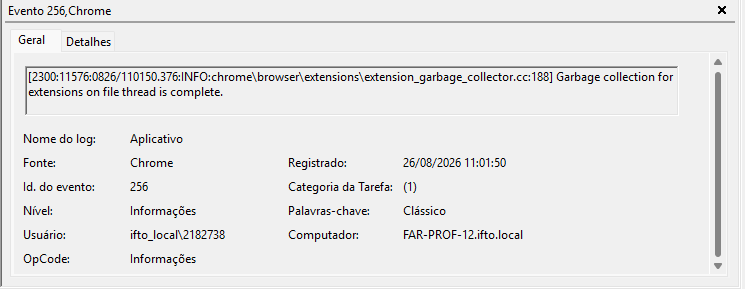
\includegraphics[scale=0.65]{chrome-event}
		\end{figure}
	\end{frame}		
	

	\begin{frame}{WinSyslog}
		\begin{figure}
			
\includegraphics[scale=0.49]{WinSyslog}
		\end{figure}
		WinSyslog is a Windows-based syslog server that receives events, 
		evaluates them through configurable rules and triggers the appropriate actions
	\end{frame}		
	
% =========================================================================================================
% logs on linux
% ==========================================================================================================
	
	\begin{frame}{Instalação e configuração dos sistemas de logs}
		\begin{itemize}
			\item JournalD
			\item Rsyslog
		\end{itemize}
		\begin{figure}
			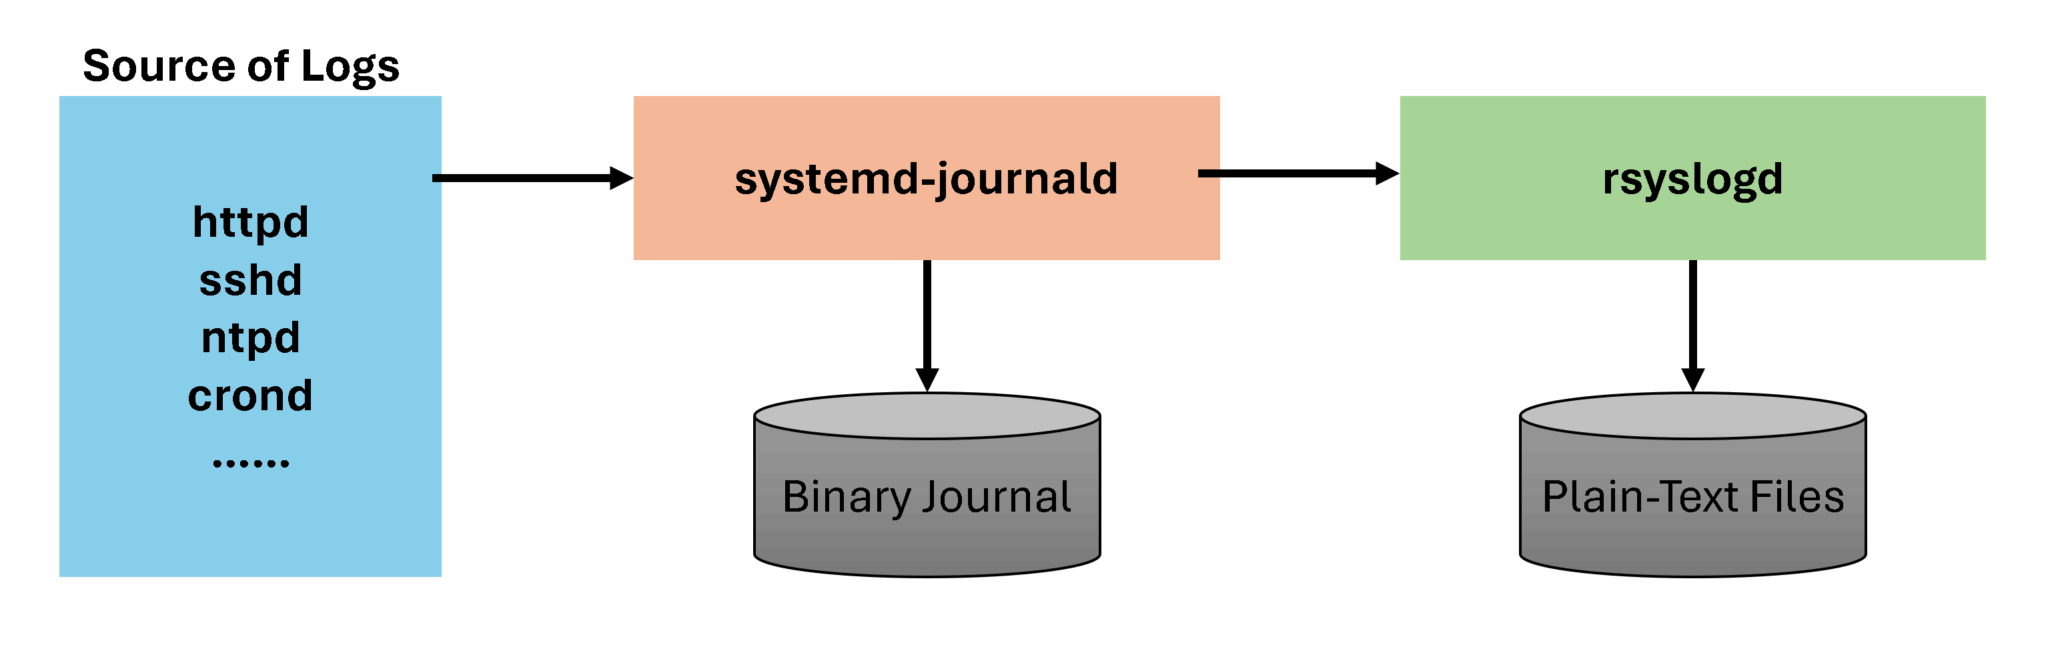
\includegraphics[scale=0.19]{journald-ryslogd}
		\end{figure}
	\end{frame}

% ============================================================
% JOURNALD – O LOG DO SYSTEMD
% ============================================================

% ============================================================
% JOURNALD – O LOG DO SYSTEMD
% ============================================================

\begin{frame}{JournalD -- O Log do Systemd}
	\begin{block}{O que é?}
		O \texttt{Journal} é um componente do SystemD que centraliza todas as mensagens registradas pelos diferentes componentes do sistema (kernel, serviços, aplicações).
	\end{block}
\end{frame}

% ============================================================

\begin{frame}{Localização dos logs}
	\begin{itemize}
		\item \textbf{Volátil:} \texttt{/run/log/journal/} (reinicia com o sistema)
		\item \textbf{Persistente:} \texttt{/var/log/journal/} (mantido após reinicializações)
	\end{itemize}
	\vspace{1em}
	
	Para ativar a persistência:
		\vspace{1em}
	
	\begin{quote}
		\texttt{sudo mkdir -p /var/log/journal}\\
		\texttt{sudo systemctl restart systemd-journald}
	\end{quote}
\end{frame}

% ============================================================

\begin{frame}{Comandos principais -- \texttt{journalctl}}
	\begin{itemize}
		\item \texttt{journalctl -u sshd} -- Logs do serviço SSH
		\item \texttt{journalctl -p err} -- Apenas erros
		\item \texttt{journalctl --since "2026-08-26 10:00"} -- A partir de uma data/hora
		\item \texttt{journalctl -f} -- Seguir em tempo real (similar ao \texttt{tail -f})
		\item \texttt{journalctl -xe} -- Detalhes estendidos para depuração
	\end{itemize}
\end{frame}

% ============================================================

\begin{frame}{Vantagens}
	\begin{itemize}
		\item Logs \textbf{indexados e estruturados} (com metadados)
		\item Metadados incluem: \textbf{PID, usuário, serviço, código-fonte}
		\item Permite busca avançada por campos
		\item Integração nativa com o SystemD
	\end{itemize}
\end{frame}

% ============================================================
% RSYSLOG – APROFUNDAMENTO
% ============================================================

\begin{frame}[allowframebreaks]{Rsyslog -- O Servidor de Logs Tradicional}
	\begin{block}{O que é?}
		O Rsyslog é um servidor de logs flexível, confiável e de alto desempenho, que coleta, filtra, roteia e armazena mensagens de log.
	\end{block}
	
	\framebreak
	
	\begin{block}{Arquitetura}
		\begin{itemize}
			\item \textbf{Inputs:} Coleta de logs (local, remoto, UDP, TCP, TLS)
			\item \textbf{Rules:} Filtros e ações baseados em facilidade/severidade
			\item \textbf{Outputs:} Destinos (arquivos, banco de dados, servidor remoto)
		\end{itemize}
	\end{block}
	
	\framebreak
	
	\begin{block}{Arquivos de configuração}
		\begin{itemize}
			\item \texttt{/etc/rsyslog.conf} -- Configuração principal
			\item \texttt{/etc/rsyslog.d/} -- Configurações específicas
		\end{itemize}
	\end{block}
	
	\framebreak
	
	\begin{block}{Instalação e serviço}
		\begin{quote}
			\texttt{sudo apt install rsyslog}\\
			\texttt{sudo systemctl status rsyslog}\\
			\texttt{sudo systemctl enable rsyslog}
		\end{quote}
	\end{block}
	
	\framebreak
	
	\begin{block}{Exemplo de configuração}
		\small
		Encaminhar logs de autenticação para um servidor remoto:
		\begin{quote}
			\texttt{auth.* @192.168.1.100:514}
		\end{quote}
		
		\vspace{0.3cm}
		Salvar logs de \texttt{sshd} em um arquivo separado:
		\begin{quote}
			\texttt{if \$programname == 'sshd' then /var/log/sshd.log}\\
			\texttt{\& stop}
		\end{quote}
	\end{block}
\end{frame}

% ============================================================
% COMPARATIVO
% ============================================================

\begin{frame}{JournalD vs Rsyslog}
	\begin{table}
		\centering
		\small
		\begin{tabular}{|p{3cm}|p{3.5cm}|p{3.5cm}|}
			\hline
			\textbf{Característica} & \textbf{JournalD} & \textbf{Rsyslog} \\
			\hline
			Origem & Nativo do SystemD & Tradicional (Syslog) \\
			\hline
			Formato & Binário (estruturado) & Texto (legível) \\
			\hline
			Filtros & Metadados (PID, usuário, etc.) & Facilidade/severidade \\
			\hline
			Persistência & Configurável & Sim (arquivos) \\
			\hline
			Log remoto & Limitado & Nativo (TCP/UDP/TLS) \\
			\hline
			Integração & SystemD & Qualquer aplicação \\
			\hline
		\end{tabular}
	\end{table}
\end{frame}
\begin{frame}	
	\begin{block}{Na prática}
		\begin{itemize}
			\item \textbf{JournalD} é usado para logs locais e depuração
			\item \textbf{Rsyslog} é usado para logs centralizados e arquiteturas complexas
		\end{itemize}
	\end{block}
\end{frame}

% ============================================================
% MÃO NA MASSA – VM DEBIAN
% ============================================================

\begin{frame}{Hands-on: Logs na VM Debian}
	\begin{block}{Atividades práticas}
		\begin{enumerate}
			\item Verifique o status do \texttt{systemd-journald}
			\item Ative a persistência dos logs do Journal
			\item Consulte logs do serviço \texttt{cups} com \texttt{journalctl}
			\item Instale o \texttt{rsyslog} (caso não esteja instalado)
			\item Configure o rsyslog para salvar logs do SSH em um arquivo separado
			\item Reinicie o serviço e teste
		\end{enumerate}
	\end{block}
\end{frame}

% ============================================================
% REFERÊNCIAS
% ============================================================

\begin{frame}[allowframebreaks]{Referências}
	\begin{thebibliography}{9}
		\bibitem{journald}
		FREEDESKTOP. \textit{Journald Documentation}. Disponível em: \url{https://www.freedesktop.org/software/systemd/man/latest/systemd-journald.service.html}. Acesso em: 26 de agosto de 2026.
		
		\bibitem{rsyslog}
		RSYSLOG. \textit{Rsyslog Documentation}. Disponível em: \url{https://www.rsyslog.com/doc/}. Acesso em: 26 de agosto de 2026.
		
		\bibitem{journalctl}
		FREEDESKTOP. \textit{journalctl Documentation}. Disponível em: \url{https://www.freedesktop.org/software/systemd/man/latest/journalctl.html}. Acesso em: 26 de agosto de 2026.
	\end{thebibliography}
\end{frame}	
\end{document}
